%Hecho por Héctor Fernando Carrera Soto | hfcarrerasoto.usac@gmail.com

\documentclass[12pt,letterpaper]{article}

\usepackage[utf8]{inputenc}
\usepackage[spanish]{babel}

%Codificación de Fuente, permite usar tildes directamente, sin ningún tipo de error.
\usepackage[T1]{fontenc}


\usepackage{amsmath}
\usepackage{amsfonts}
\usepackage{amssymb}
\usepackage{graphicx}
\usepackage[left=2.5cm,right=1.5cm,top=1.5cm,bottom=1.5cm]{geometry}

%Para tachar dimencionales usar \cancel
\usepackage{cancel}

%>>>>>>>>>>>>>><Fuente parecido al arial<<<<<<<<<<<
\usepackage{helvet}
\renewcommand*\familydefault{\sfdefault}



\usepackage[pdftex]{hyperref}


%<<<<<<<<< para saltos de página usar  \clearpage >>>>>
%<<<<<<<<< para saltos entre líneas usar \vspace{2cm}>>>>>
%<<<<<<<<< para espaciado horizontal \hspace{1cm}>>>>>
%<<<<<<<<< para colocar url o referencias a url usar \url{http://www.latex-project.org/} o  \href{http://www.latex-project.org/}{latex project}>>>>>>>}

%Texto al azar
\usepackage{lipsum}

%Arreglar figuras
\usepackage{float}


%Sangría
\setlength{\parindent}{0pt}
\usepackage{cancel}
\spanishdecimal{.}

\usepackage{multicol}

%\frontmatter Se supone que se refiere a las partes previas al cuerpo del libro propiamente dicho: prólogo, introducción, índices. Si introducimos ese comando al principio del fichero haremos que las páginas se numeren en números romanos y que el comando \chapter no incluya el número ni la palabra "Capítulo" (como ocurriría si usáramos \chapter*), pero sí incluya el título en el índice (cosa que no ocurriría de usar \chapter*).

%\mainmatter Con este comando le indicamos a LaTeX que ha terminado la parte inicial y a continuación viene el libro propiamente dicho. Hay que usarlo cuando se ha usado previamente \frontmatter. El efecto de \mainmatter es que se reinicia la numeración de las páginas, que pasan además a volver a numerarse con números arábigos. El comando \chapter vuelve además a su comportamiento habitual.

%\backmatter se debe usar (si se usa) al final del documento. Provoca que \chapter funcione igual que en \frontmatter, pero no afecta a la numeración de las páginas.

%<<<<<<<<< Comando valores absolutos |x| >>>>>
\providecommand{\abs}[1]{\lvert1\rvert}
%<<<<<<<<< Comando para la normal ||x|| >>>>>
\providecommand{\norm}[1]{\lVert1\rVert}

%<<<<<<<<< para saltos de página usar  \clearpage >>>>>
%<<<<<<<<< para saltos entre líneas usar \vspace{2cm}>>>>>
%<<<<<<<<< para espaciado horizontal \hspace{1cm}>>>>>
%<<<<<<<<< para colocar url o referencias a url usar \url{http://www.latex-project.org/} o  \href{http://www.latex-project.org/}{latex project}>>>>>>>


%<<<<<<<<< Configuraciónes en las tablas >>>>>
%Paquete para configurar medidas de las tablas
\usepackage{tabularx}
%Forma del comando
%\begin{tabular}{|m{0.22\linewidth}|m{0.22\linewidth}|}


%<<<<<<<<< Para configurar \begin{enumerate}[A)]  en donde está la letra "A" escogemos como queremos enumerar, ejemplo \begin{enumerate}[i)]>>>>>>>>>>>>>>
\usepackage{enumerate}

\usepackage{multirow}
\usepackage{balance}
\begin{document}

%%%%%%%%%%%%%%%%%
%	Encabeado	%
%%%%%%%%%%%%%%%%%

\begin{title}

\begin{table}[H]
\begin{center}
\begin{tabular}{|c|m{0.20\linewidth}|c|m{0.10\linewidth}|}
\multirow{4}{*}{
\includegraphics[scale=0.3]{EIME.png}}                                                         & \multicolumn{3}{l}{Ingeniería electrónica}                                       \\
                                                                                & \multicolumn{3}{l}{Proyectos computacionales aplicados a ingeniería electrónica} \\
                                                                                & \multicolumn{3}{l}{Ing. José Anibal Silva de Los Angeles}                        \\
                                                                                & \multicolumn{3}{l}{Aux. Fernando Mardoqueo Paxtor Sam}                           \\ \hline 
	\multicolumn{1}{|l|}{Carné:} & 201700923 & Fecha: & \multicolumn{1}{l|}{15/2/2022}\\ 
	\hline 
	\multicolumn{1}{|l|}{Nombre:} & \multicolumn{3}{l|}{Héctor Fernando Carrera Soto} \\ 
	\hline 
	\multicolumn{1}{|l|}{Registro admin:} & \multicolumn{3}{l|}{3505043180101} \\ 
	\hline 
	\end{tabular} 
\end{center}
\end{table}

\end{title}

%%%%%%%%%%%%%%%%%%%%%%%%%%%%%%%%%%%%%%%%%
%	Escriba su tarea aquí abajo prro :v	%
%%%%%%%%%%%%%%%%%%%%%%%%%%%%%%%%%%%%%%%%%

\section{Creando y actualizando repositorio}



\begin{multicols}{2}

\begin{figure}[H]
\centering
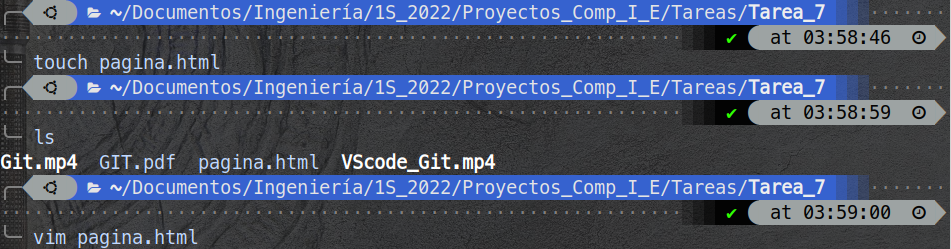
\includegraphics[width = \columnwidth]{Git_1.png}
\caption{Paso 1.}
\end{figure}

\begin{figure}[H]
\centering
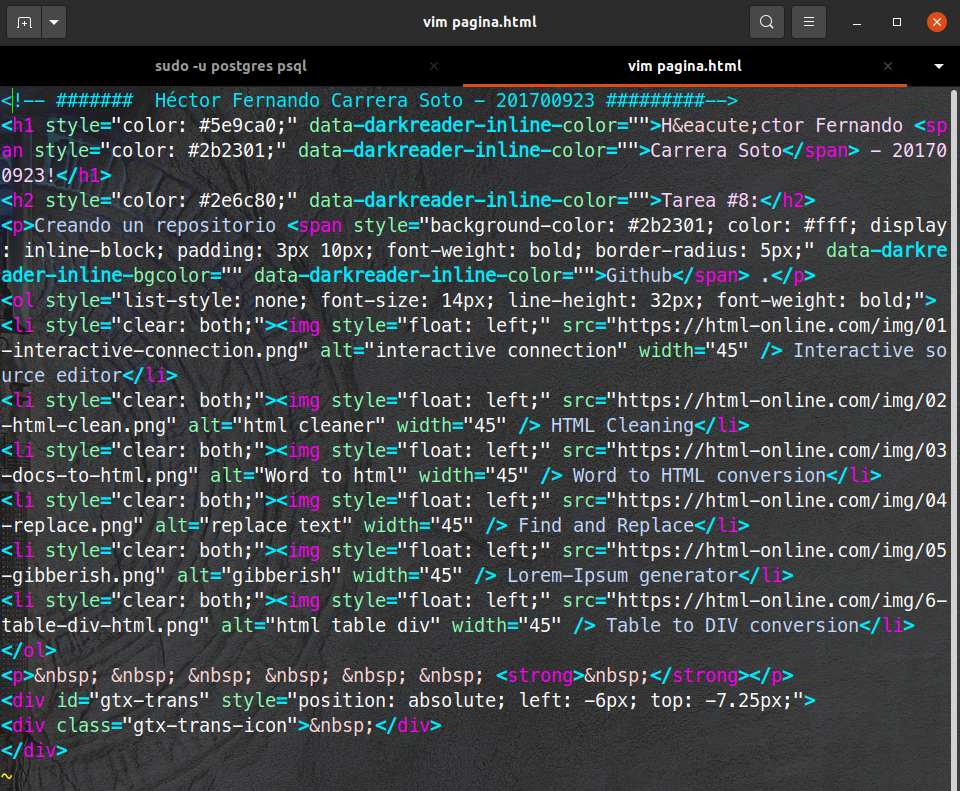
\includegraphics[width = \columnwidth]{Git_2.png}
\caption{Paso 2.}
\end{figure}


\begin{figure}[H]
\centering
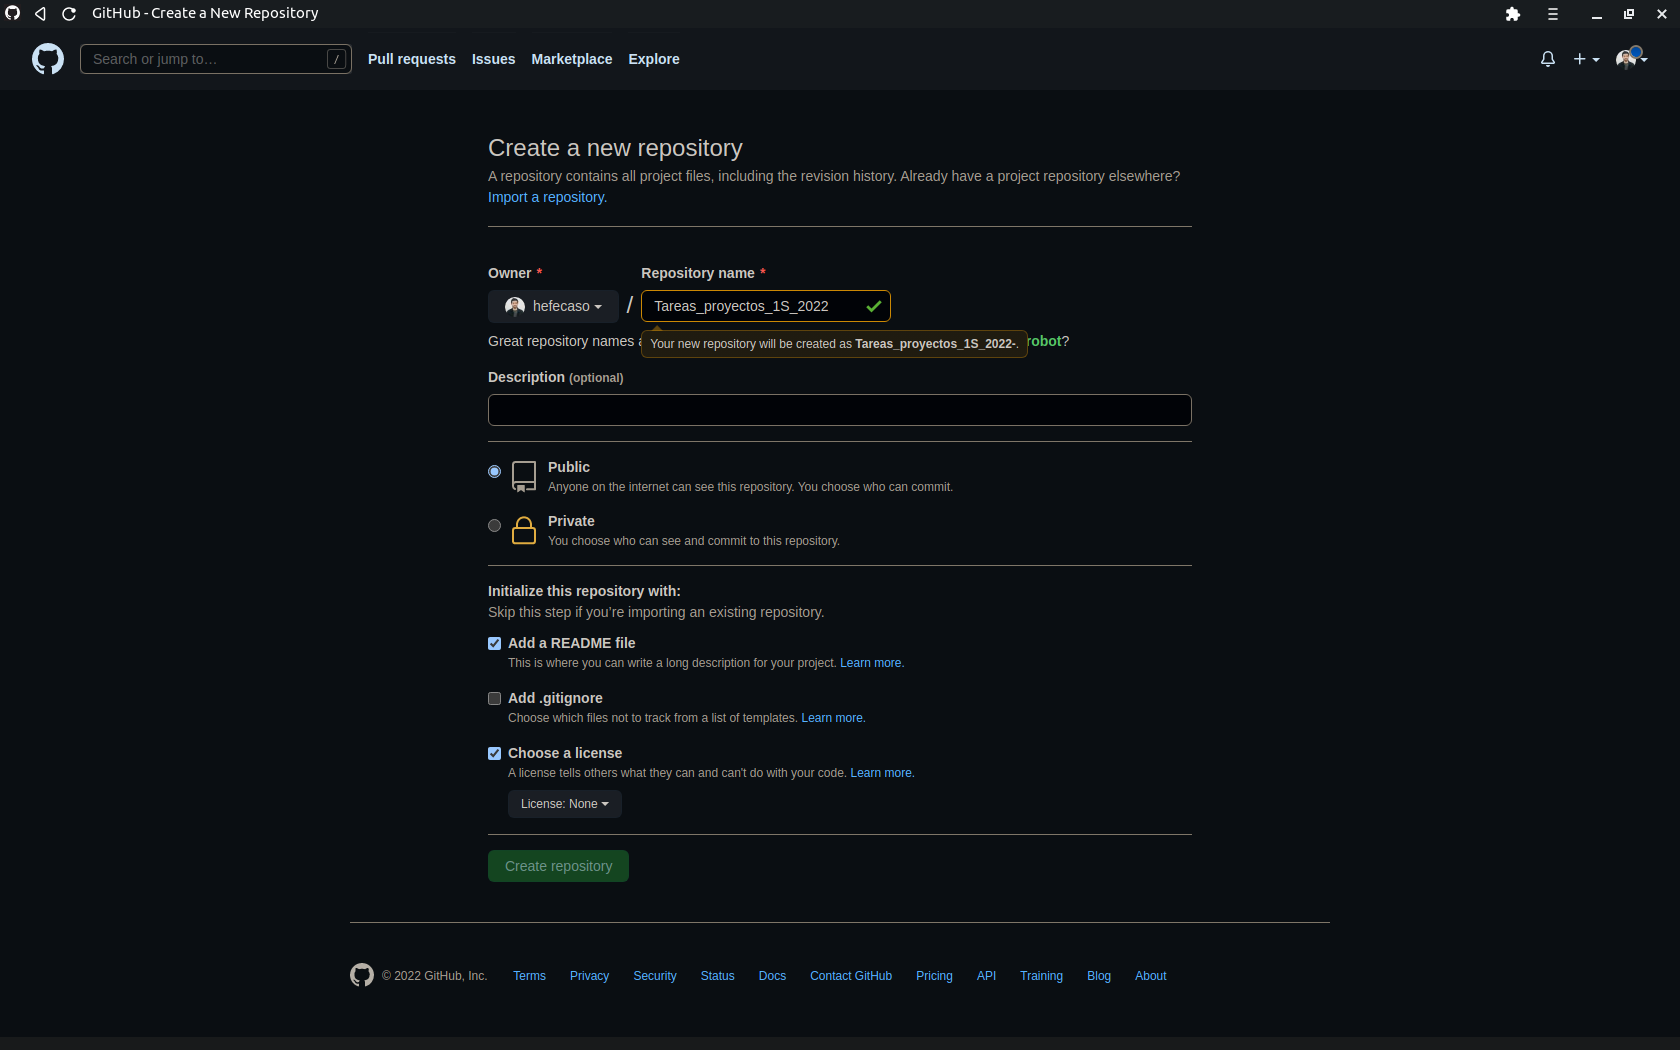
\includegraphics[width = \columnwidth]{Git_3.png}
\caption{Paso 3.}
\end{figure}


\begin{figure}[H]
\centering
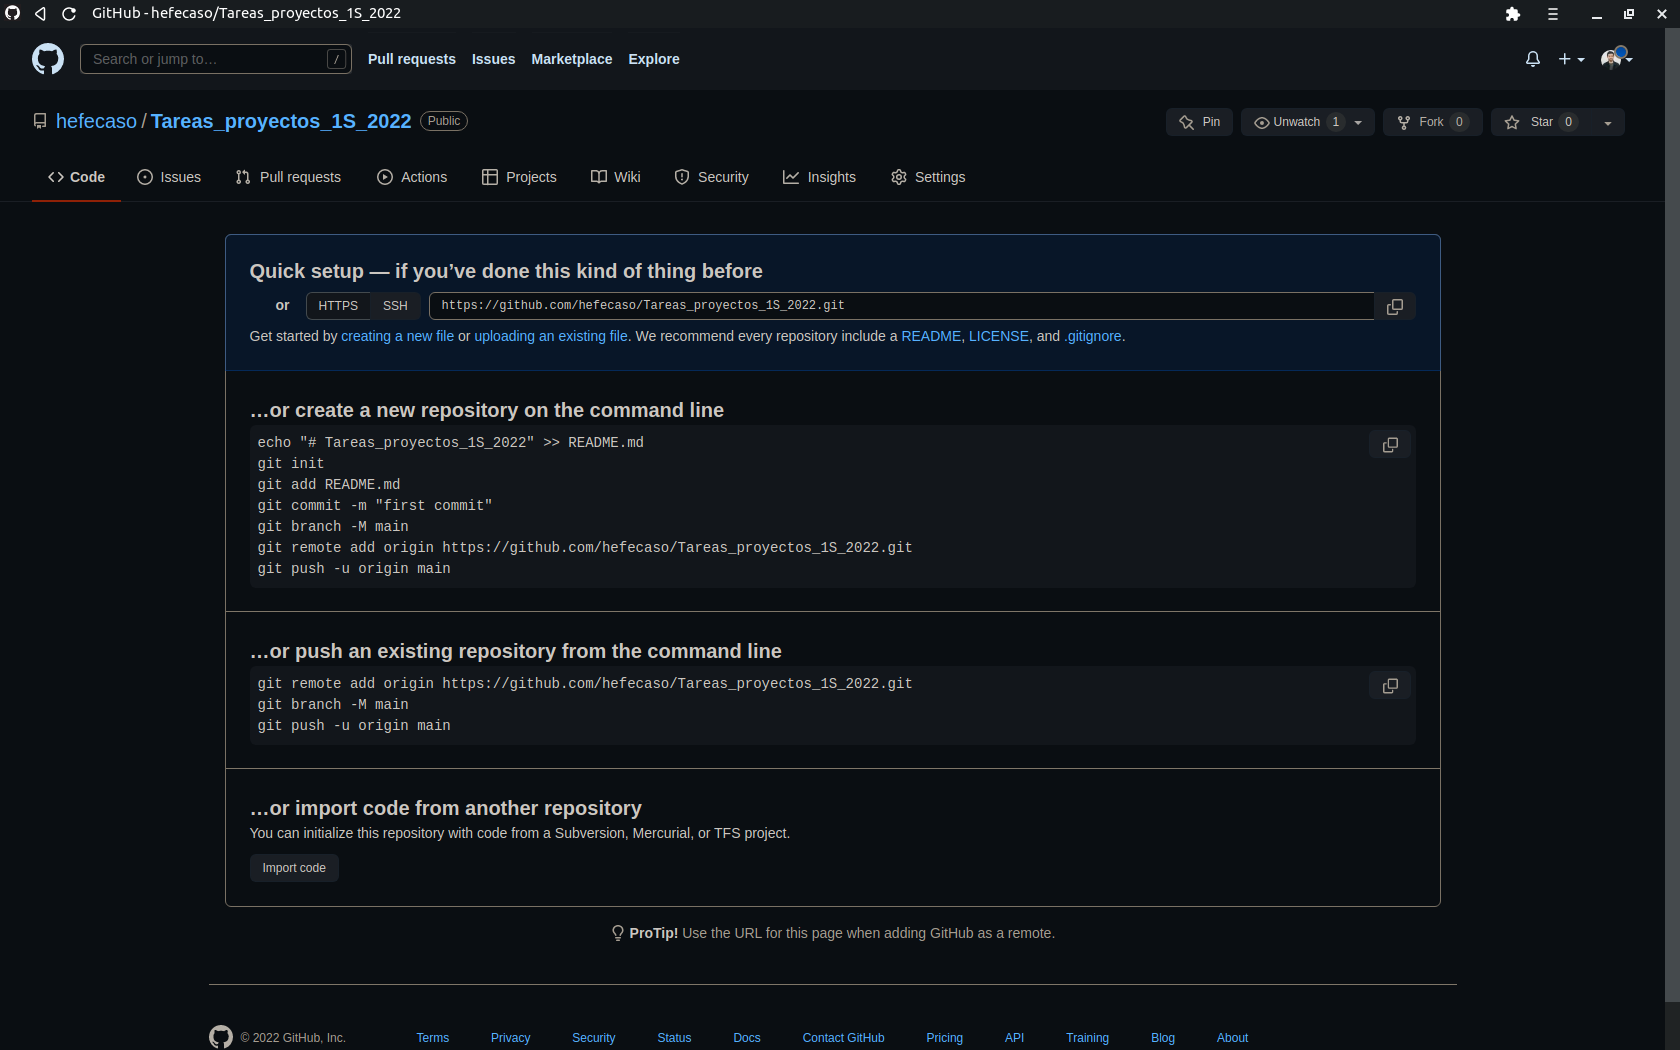
\includegraphics[width = \columnwidth]{Git_4.png}
\caption{Paso 4.}
\end{figure}

\begin{figure}[H]
\centering
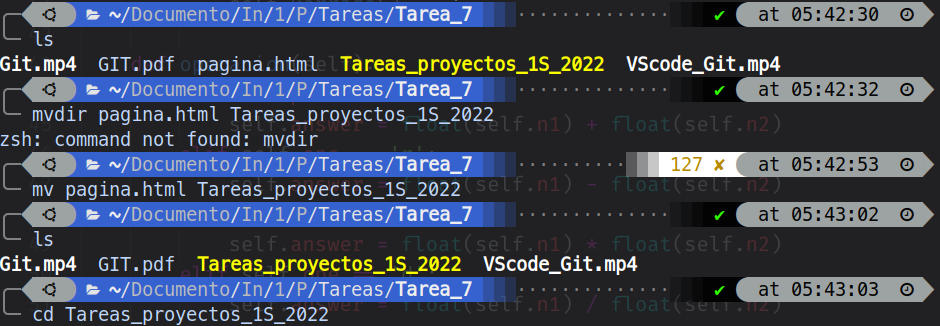
\includegraphics[width = \columnwidth]{Git_5.png}
\caption{Paso 5.}
\end{figure}


\begin{figure}[H]
\centering
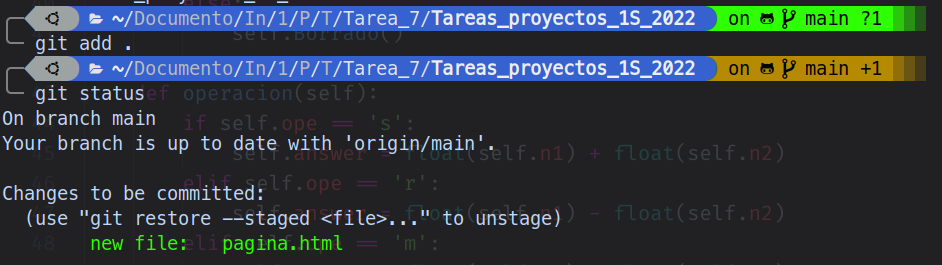
\includegraphics[width = \columnwidth]{Git_6.png}
\caption{Paso 6.}
\end{figure}


\begin{figure}[H]
\centering
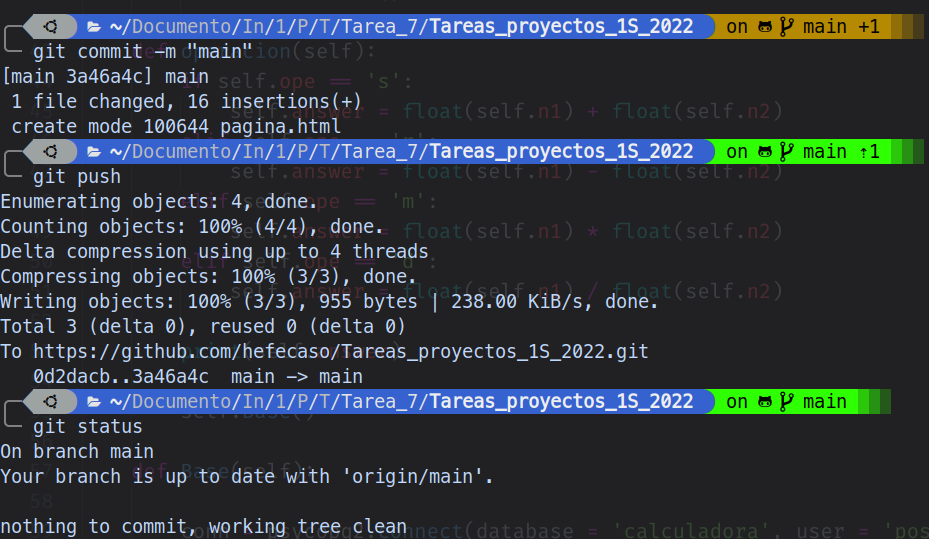
\includegraphics[width = \columnwidth]{Git_7.png}
\caption{Paso 7.}
\end{figure}



\begin{figure}[H]
\centering
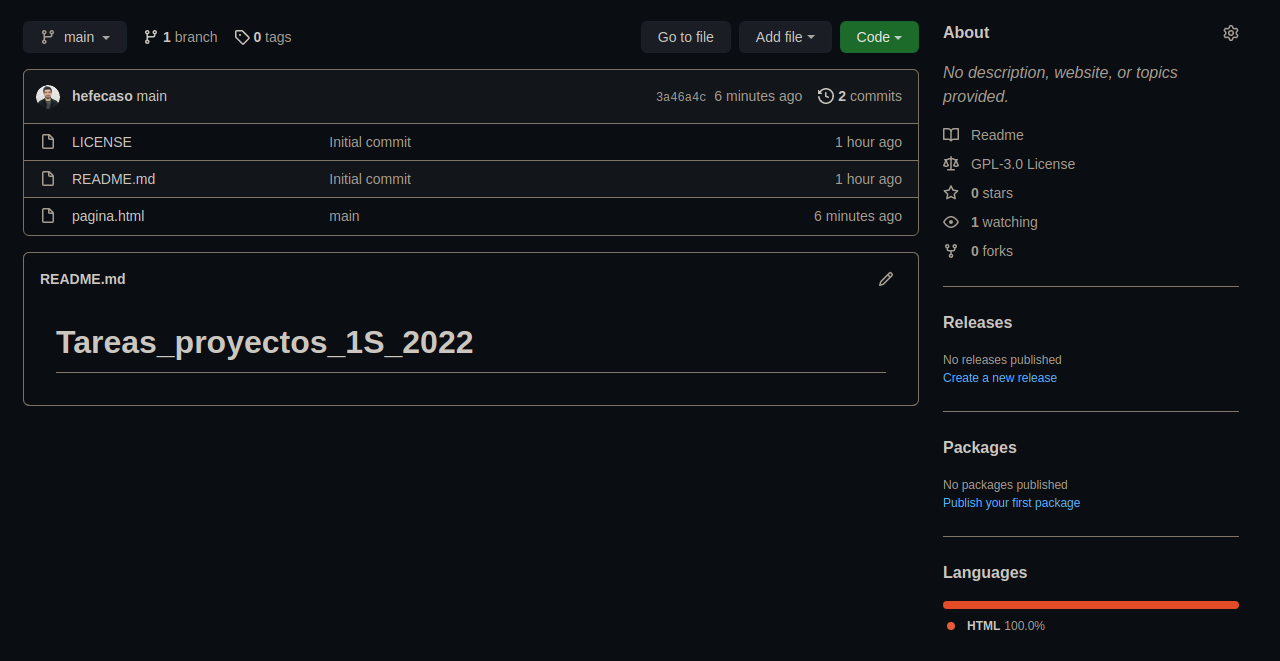
\includegraphics[width = \columnwidth]{Git_8.png}
\caption{Paso 8.}
\end{figure}

\section{Enlace a Github}

\url{https://github.com/hefecaso/0980_Proyectos_de_computacion_aplicada_a_IE_1S_2022.git}

\end{multicols}
\balance
\end{document}
